%%%%%%%%%%%%%%%%%%%%%%%%%%%%%%%%%%%%%%%%%%%%%%%%%%%%%%%%%%%%%%%%%
% Dissertacao de Mestrado / Dept Fisica, CFM, UFSC              %
% Andre@UFSC - 2011                                             %
%%%%%%%%%%%%%%%%%%%%%%%%%%%%%%%%%%%%%%%%%%%%%%%%%%%%%%%%%%%%%%%%%


%:::::::::::::::::::::::::::::::::::::::::::::::::::::::::::::::%
%                                                               %
%                          Capítulo 4                           %
%                                                               %
%:::::::::::::::::::::::::::::::::::::::::::::::::::::::::::::::%

%***************************************************************%
%                                                               %
%                       Análise da Amostra                      %
%                                                               %
%***************************************************************%

\chapter{Análise da amostra \STARLIGHTUV}
\label{sec:Analise}


%***************************************************************%
%                                                               %
%                  Análise - Diagrama cor -- cor                %
%                                                               %
%***************************************************************%

\section{Diagrama cor--cor}

De posse de uma amostra de galáxias com uma informação adicional (as magnitudes
em ultravioleta), é natural tentar ver como estas novas medidas se relacionam às
medidas conhecidas. \citet{Chilingarian2011} mostram que, num gráfico
tridimensional das cores $\mathrm{NUV}-r$ e $g-r$ contra a magnitude $z$, a
distribuição de galáxias pode ser aproximada por uma superfície polinomial de
baixa ordem. Os autores mostram que há uma forte correlação entre a cor
$\mathrm{NUV}-r$ e a morfologia da galáxia. Eles também estudam o histórico de
formação estelar (SFH) no diagrama $\mathrm{NUV}-r$ contra $g-r$ (diagrama
cor--cor), mas a exploração é um tanto superficial.

\begin{figure}
	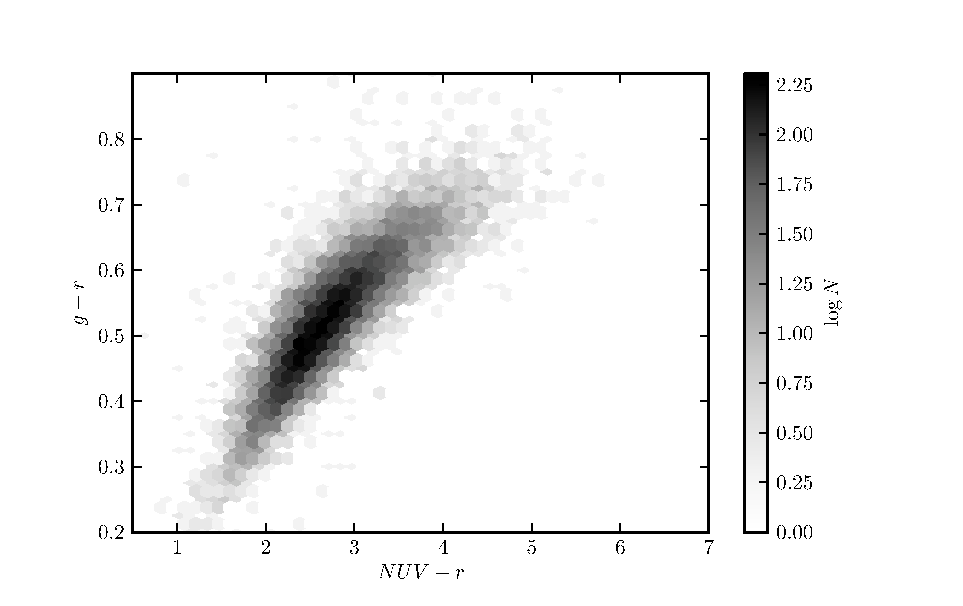
\includegraphics{figuras/uvcolor-color-density.eps}
	\caption[Frequência de galáxias no diagrama cor--cor.]
	{Frequência de galáxias no diagrama cor--cor ($\mathrm{NUV}-r$ {\em versus}
	$g-r$) da amostra \starlightUV.}
	\label{fig:DensityColor}
\end{figure}

O diagrama cor--cor para a amostra \starlightUV é mostrado na Figura
\ref{fig:DensityColor}. A cor das caixas hexagonais representa o logaritmo do
número de galáxias. Através das curvas de nível é possível ver a bimodalidade da
distribuição, separando as galáxias nas sequências vermelha e azul. A Figura
\ref{fig:ColorStarlightParam} mostra as propriedades físicas das galáxias
obtidas através do \starlight no diagrama cor--cor. Os eixos são os mesmos da
Figura \ref{fig:DensityColor}, com a cor dos pontos indicando o valor de cada
parâmetro. \citeauthor{Chilingarian2011} chegam numa relação semelhante à do
painel (a) para a idade estelar das galáxias, porém através de outros meios.
Estas propriedades físicas são vistas com mais detalhes na Seção
\ref{sec:Analise:PropFisicas}.

\begin{figure}
	\includegraphics{figuras/uvcolor-color.eps}
	\caption[Diagrama cor--cor para os diversos parâmetros \starlight.]
	{Propriedades físicas das galáxias em função de cor UV e cor óptica. Os
	contornos das figuras representam os níveis referentes à Figura
	\ref{fig:DensityColor}, e os eixos horizontal e vertical são os mesmos
	utilizados naquela figura. As cores dos pontos nos painéis correspondem a:
	\textbf{(a)} Média do logaritmo da idade das SSP componentes da galáxia,
	ponderada pelo fluxo. \textbf{(b)} O mesmo que a anterior, mas ponderada pela
	massa. \textbf{(c)} Metalicidade média das SSP componentes da galáxia,
	ponderada pelo fluxo. \textbf{(d)} O mesmo que a anterior, ponderada pela
	massa. \textbf{(e)} Logaritmo da massa estelar da galáxia, em massas solares.
	\textbf{(f)} Atenuação por poeira na galáxia, na banda $V$.}
	\label{fig:ColorStarlightParam}
\end{figure}


%***************************************************************%
%                                                               %
%                     Análise - Classificação                   %
%                                                               %
%***************************************************************%

\section{Classificação das galáxias}

Nesta seção são discutidas formas de classificação de galáxias e a forma como a
cor UV das galáxias está relacionada às classes. São utilizadas as linhas de
emissão \Halpha, \Hbeta, \NII e \OIII (daqui em diante chamados apenas de \nII e
\oIII).

A classificação feita a seguir divide as galáxias em dois grupos principais: as
galáxias com linha de emissão (ELG) e as galáxias passivas (PG). As ELG ainda
podem ser divididas dependendo do processo físico por trás das linhas de
emissão. Essencialmente, os agentes ionizantes responsáveis pelas linhas
observadas em galáxias são estrelas jovens, núcleos ativos e objetos do tipo
HOLMES ({\em Hot Low-Mass Evolved Stars}). \citet{CidFernandes2011} elabora um
procedimento simples para separar as galáxias em classes, de acordo com o agente
ionizante que domina a emissão de linhas na galáxia. A distinção é feita de
acordo com a largura equivalente da linha \Halpha ($\WHa$) e a razão entre o
fluxo de linhas $\nII/\Halpha$, num diagrama conhecido como WHAN. Este diagrama
relaciona duas quantidades físicas diferentes: $\WHa$ mede a quantidade de
fótons ionizantes em relação à massa estelar, e $\nII/\Halpha$ mede a abundância
de nitrogênio, o estado de ionização e a temperatura do gás. Assim, as galáxias
são separadas em classes neste diagrama conforme os seguintes critérios:

\begin{list}{}{\setlength\itemsep{0pt}}
\item \textbf{(a)} Galáxias com formação estelar (SF): $\log(\nII/\Halpha) <
-0,4$ e $\WHa > 3\,\text{\AA}$,
\item \textbf{(b)} Galáxias com núcleo ativo forte (sAGN): $\log(\nII/\Halpha) >
-0,4$ e $\WHa > 6\,\text{\AA}$,
\item \textbf{(c)} Galáxias com núcleo ativo fraco (wAGN): $\log(\nII/\Halpha) >
-0,4$ e $3\,\text{\AA} > \WHa > 6\,\text{\AA}$,
\item \textbf{(d)} Galáxias ``aposentadas'' (RG): $0,5\,\text{\AA} < \WHa <
3\,\text{\AA}$,
\item \textbf{(e)} Galáxias passivas (PG): $\WHa < 0,5\,\text{\AA}$ e $\WnII <
0,5\,\text{\AA}$.
\end{list}

Neste esquema, as SF têm linhas de emissão devido a estrelas jovens e massivas,
as sAGN e wAGN têm linhas devido a núcleos ativos, as RG têm linhas devido a
HOLMES e as PG não têm emissão mensurável.

O diagrama WHAN para a amostra \starlightUV pode ser visto na Figura
\ref{fig:Whan}. A cor dos pontos para cada classe é a mesma utilizada por
\citet{CidFernandes2011}. São $42\,694$ galáxias com formação estelar, $32\,193$
galáxias com núcleo ativo forte, $11\,972$ galáxias com núcleo ativo fraco,
$24\,385$ galáxias aposentadas e $13\,425$ galáxias passivas. O mesmo diagrama,
porém com a cor dos pontos representando a cor $\mathrm{NUV}-r$ das galáxias
(Figura \ref{fig:WhanUV}), mostra que a cor UV das galáxias está relacionada à
sua classe.

\begin{figure}
	\includegraphics{figuras/whan.eps}
	\caption[Diagrama de diagnóstico WHAN.]
	{Diagrama de diagnóstico WHAN. As linhas tracejadas separam as galáxias
	em classes. \textbf{Azul}: galáxias com formação estelar (SF). \textbf{Verde
	claro}: galáxias com núcleo ativo forte (sAGN). \textbf{Verde forte}:
	galáxias com núcleo ativo fraco (wAGN). \textbf{Preto}: galáxias aposentadas
	(RG). \textbf{Vermelho}: galáxias passivas (PG). \textbf{Magenta}: Galáxias
	que não se encaixam em nenhuma destas classes.}
	\label{fig:Whan}
\end{figure}

\begin{figure}
	\includegraphics{figuras/whan-uv.eps}
	\caption[Cores UV no diagrama WHAN.]
	{Diagrama WHAN semelhante ao da Figura \ref{fig:Whan}. A cor dos pontos
	representa $\mathrm{NUV}-r$. Pode-se notar que a cor UV das galáxias é
	diferente para cada classe.}
	\label{fig:WhanUV}
\end{figure}

Outra forma de classificar as galáxias é através das razões entre linhas de
emissão $\nII/\Halpha$ e $\oIII/\Hbeta$. Este diagrama, conhecido como BPT
\citep*{Baldwin1981} é bastante utilizado na astronomia extragalática. Em
\citet{CidFernandes2010}, discute-se os detalhes da classificação das galáxias
utilizando o diagrama BPT. As linhas tracejadas separam as galáxias nas classes
{\em Seyfert} (que corresponde à classe sAGN na classificação pelo WHAN), {\em
LINER}\footnote{{\em Low-Ionization Nuclear Emission-Line Region}: região
nuclear com linhas de emissão de baixa ionização.} (correspondente às wAGN e
aposentadas) e galáxias com formação estelar (SF). A cor UV das galáxias da
amostra no diagrama BPT (Figura \ref{fig:BPTUV}) é consistente com as cores para
o diagrama WHAN.

\begin{figure}
	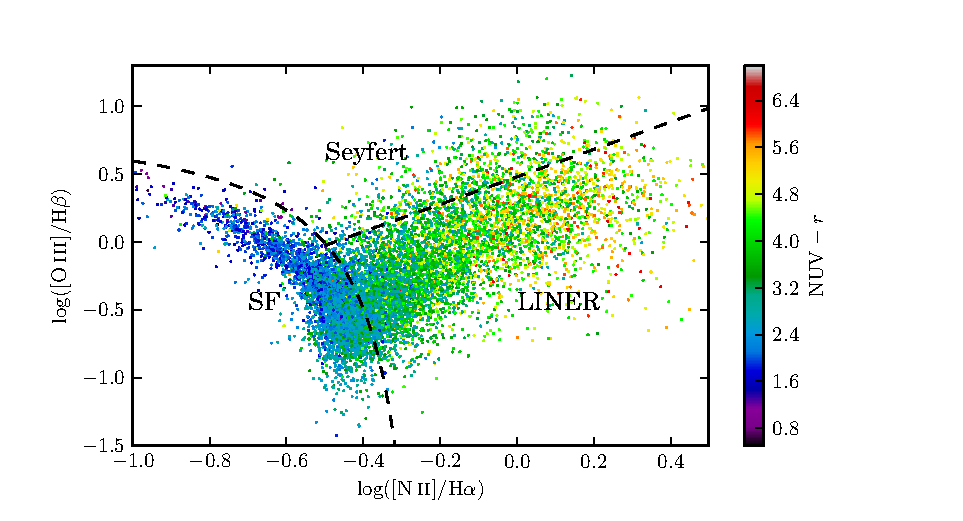
\includegraphics{figuras/bpt-uv.eps}
	\caption[Cores UV no diagrama BPT.]
	{Diagrama BPT, também usado para classificar galáxias. A cor dos
	pontos representa $\mathrm{NUV}-r$. As linhas tracejadas separam das galáxias nas
	classes {\em Seyfert}, {\em LINER} e formação estelar, conforme
	\citet[linhas S06 e K06 da tabela 1]{CidFernandes2010}. As classes possuem
	cores UV consistentes com a classificação proveniente do diagrama WHAN.}
	\label{fig:BPTUV}
\end{figure}

\begin{figure}
	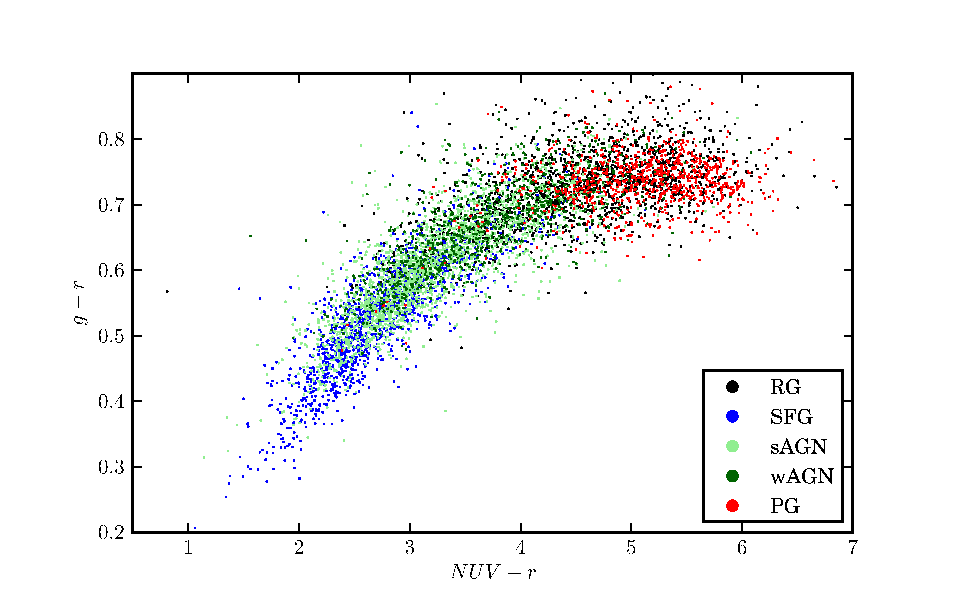
\includegraphics{figuras/uvcolor-color-class.eps}
	\caption[Diagrama cor--cor UV de acordo com o tipo de galáxia.]
	{Classes de galáxias no diagrama cor--cor UV. As cores referentes às classes de
	galáxia são as mesmas do diagrama WHAN (Figura \ref{fig:Whan}). É possível
	notar uma separação entre as classes, embora haja uma sobreposição severa
	entre elas.}
	\label{fig:ColorClass}
\end{figure}

\begin{figure}
	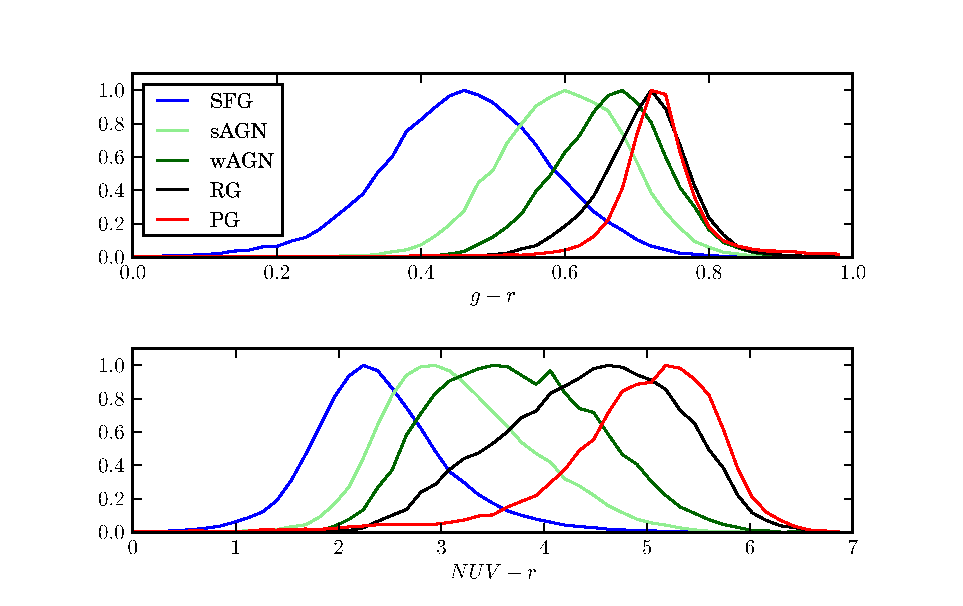
\includegraphics{figuras/histo_galtype_color.eps}
	\caption[Histogramas de cores para as classes de galáxias.]
	{Histogramas normalizados das cores óptica ($g-r$) e ultravioleta
	($\mathrm{NUV}-r$) para as classes de galáxias. A cor das linhas representa a
	classe conforme a Figura \ref{fig:Whan}. Em ultravioleta aparece uma separação
	entre as classes de galáxias aposentadas (RG) e passivas (PG). Note que os
	histogramas seguem o agrupamento das classes na Figura
	\ref{fig:ColorClass}.}
	\label{fig:HistogramaCorClasse}
\end{figure}

As classes de galáxias ocupam regiões distintas do diagrama cor--cor na Figura
\ref{fig:ColorClass}. A cor dos pontos representa a classe das galáxias
utilizando o mesmo código de cores da Figura \ref{fig:Whan}. Embora não esteja
muito claro para as RG e PG, as classes formam uma sequência neste diagrama.
Isto pode ser visto mais facilmente na Figura \ref{fig:HistogramaCorClasse}.
Esta figura é de certo modo uma versão resumida da Figura \ref{fig:ColorClass}.
Mesmo havendo uma sobreposição considerável entre as classes, a sequência está
bem definida.

É interessante notar que a separação entre as classes é mais pronunciada em UV.
As classes RG e PG mal se distinguem no óptico, enquanto que em UV as RG se
mostram consistentemente mais azuis\footnote{O conceito de ``mais azul'' não
está relacionado à percepção de cor, mas sim ao fato de que um objeto emite mais
luz em comprimentos de onda menores.}. Através de uma inspeção visual pode-se
inferir, ainda que qualitativamente, que as distribuições em UV são
significativamente assimétricas em comparação com as distribuições no óptico.
Isto pode ser indício de uma contaminação entre as classes, evidenciada agora
pelos novos dados em UV.

O mesmo pode ser dito sobre as distribuições de galáxias RG e wAGN, cuja
diferença no óptico é magnificada em $\mathrm{NUV}-r$, embora, como no caso das
RG e PG, persista uma grande superposição. Isto não é surpreendente, já que as
classes são definidas de modo completamente independente das cores ópticas e UV.
Além disso, qualquer linha divisória entre uma classe e outra é inevitavelmente
difusa, devido a erros observacionais e ao próprio fato de que os fenômenos que
representam duas classes podem coexistir. Nada impede, por exemplo, que uma
galáxia seja aposentada, no sentido de não formar mais estrelas, e possua um
núcleo ativo fraco alimentando-se de tão pouco gás que não seja suficiente para
formar estrelas.

\begin{figure}
	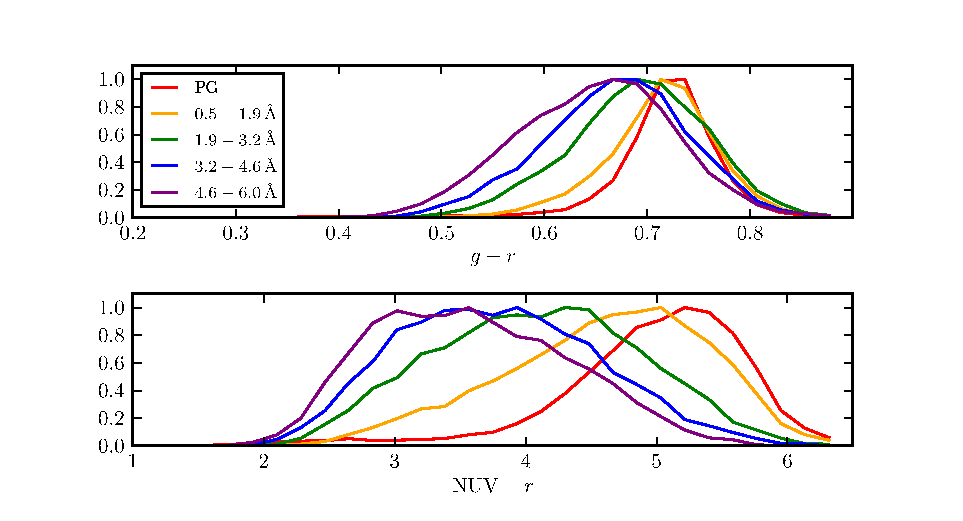
\includegraphics{figuras/histo_wha_color.eps}
	\caption[Histogramas de cores em função de \WHa.]
	{Histogramas normalizados das cores óptica ($g-r$) e ultravioleta
	($\mathrm{NUV}-r$) para várias faixas de \WHa. Para comparação, é mostrado (em
	vermelho) também o histograma para as PG. Foram selecionadas galáxias com
	$\log(\nII/\Halpha) < -0,4$ e $0,5\,\text{\AA} < \WHa < 6\,\text{\AA}$, ou
	seja, todas as galáxias wAGN e RG.}
	\label{fig:HistogramaCorWHa}
\end{figure}

\begin{figure}
	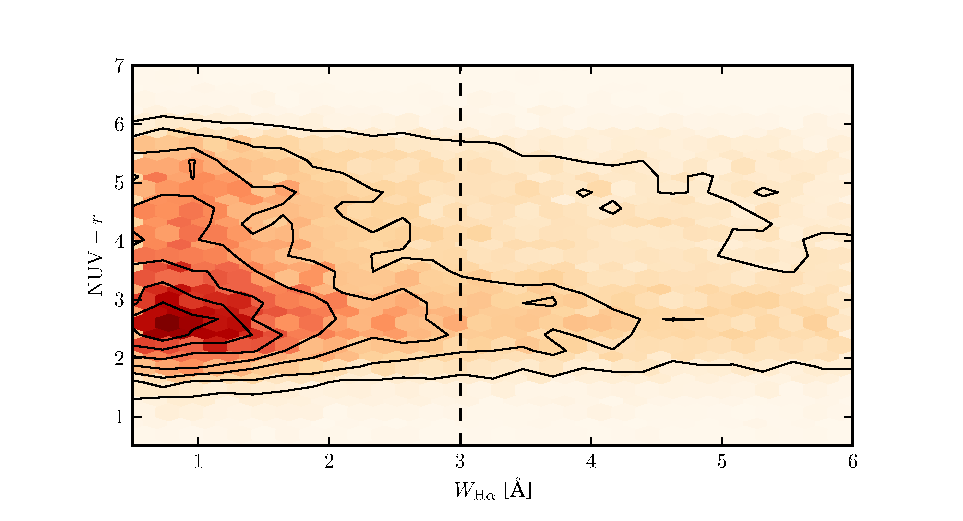
\includegraphics{figuras/wha_nuv.eps}
	\caption[Cor UV em função de \WHa.]
	{Frequência de galáxias em função da cor UV e de \WHa para as mesmas
	galáxias da figura \ref{fig:HistogramaCorWHa}, ou seja, $\log(\nII/\Halpha) <
	-0,4$ e $0,5\,\text{\AA} < \WHa < 6\,\text{\AA}$. A linha tracejada indica a
	fronteira entre RG ($\WHa < 3\,\text{\AA}$) e wAGN ($\WHa > 3\,\text{\AA}$)}
	\label{fig:ColorWha}
\end{figure}

Para apreciar com um pouco mais de detalhe a diferença em UV entre as galáxias
das classes wAGN, RG e PG, a Figura \ref{fig:HistogramaCorWHa} repete os
histogramas da Figura \ref{fig:HistogramaCorClasse}, mas desta vez limitada a
objetos com $\log(\nII/\Halpha) > -0.4$ e $\WHa < 6\,\text{\AA}$, excluindo,
portanto, galáxias SF e sAGN. As diferentes cores representam faixas em \WHa,
com uma quantidade de subdivisões suficiente para mostrar a tendência sem
comprometer a clareza. O que se observa na figura é uma progressão gradual e
unívoca na direção de cores mais vermelhas a medida em que \WHa diminui. As
galáxias RG mais azuis são aquelas que têm os maiores valores de \WHa permitidos
para esta classe ($\WHa < 3\,\text{\AA}$). De modo similar, as galáxias wAGN que
têm \WHa próximo à fronteira entre wAGN e RG são aqueles com cores mais
vermelhas. Esses resultados também podem ser vistos na Figura
\ref{fig:ColorWha}, onde as mesmas galáxias são apresentadas em um diagrama
$\mathrm{NUV}-r$ contra \WHa.

Estas figuras corroboram a suspeita levantada acima de que a superposição em
$\mathrm{NUV}-r$ entre classes espectrais definidas com base em \WHa é, em
grande medida, devida ao conflito entre uma descrição discreta e uma realidade
contínua. Neste caso limites rígidos de classificação têm apenas um sentido
estatístico. Ao mesmo tempo, na medida em que revelam uma correlação entre \WHa
e $\mathrm{NUV}-r$, as Figuras \ref{fig:HistogramaCorWHa} e \ref{fig:ColorWha}
reforçam o uso de \WHa como uma propriedade observacional útil para
classificação. Como salientado por \citet{CidFernandes2011}, o uso de uma
largura equivalente vai contra a história da classificação espectral baseada em
linhas de emissão (baseada exclusivamente em razões de fluxos), mas é a única
maneira de separar AGNs verdadeiros de falsos.


%***************************************************************%
%                                                               %
%         Análise - Prop. Físicas no diagrama cor -- cor        %
%                                                               %
%***************************************************************%

\section{Propriedades físicas no diagrama cor--cor}
\label{sec:Analise:PropFisicas}

Os agentes por trás das linhas de emissão das galáxias são fundamentalmente
diferentes (estrelas jovens, núcleos ativos e HOLMES) para cada classe. Não é de
se estranhar, portanto, que as propriedades físicas das galáxias estejam
relacionadas à sua classificação.

\begin{figure}
	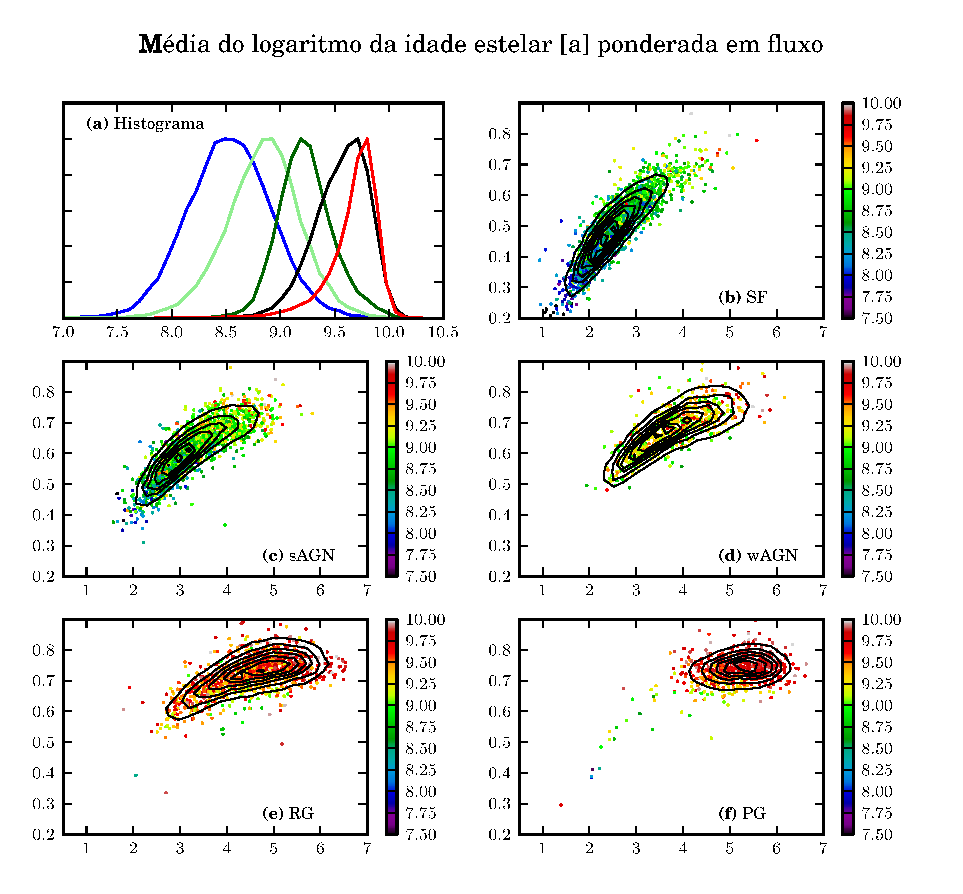
\includegraphics{figuras/uvcolor-color-at_flux-byclass.eps}
	\caption[Idade estelar média ponderada em fluxo no diagrama cor--cor.]
	{Média do logaritmo da idade estelar das galáxias, ponderada pelo fluxo, em
	função de $\mathrm{NUV}-r$ e $g-r$. O painel \textbf{(a)} mostra o histograma
	normalizado das idades para cada classe, utilizando o mesmo código de cores da
	Figura \ref{fig:Whan}. Os painéis de \textbf{(b)} a \textbf{(f)} são diagramas
	cor--cor com eixos iguais aos da Figura \ref{fig:DensityColor} código de cor
	indicando a idade, contendo somente as galáxias com formação estelar (SF), AGN
	fortes (sAGN), AGN fracas (wAGN), galáxias aposentadas (RG) e galáxias passivas
	(PG), respectivamente. Os contornos indicam a densidade de galáxias.}
	\label{fig:ATFluxColor}
\end{figure}

\begin{figure}
	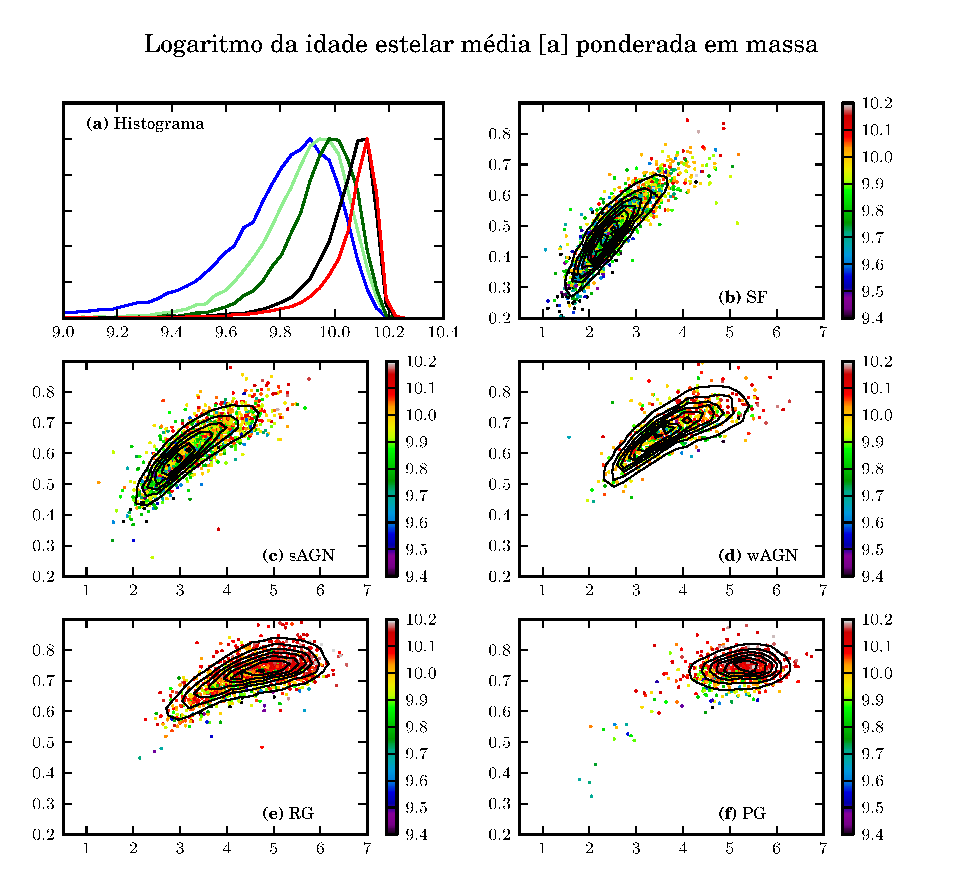
\includegraphics{figuras/uvcolor-color-at_mass-byclass.eps}
	\caption[Idade estelar média ponderada em massa no diagrama cor--cor.]
	{O mesmo que a Figura \ref{fig:ATFluxColor}, para a média do logaritmo da idade
	estelar das galáxias, ponderada pela massa. Note que a escala de idades não é a
	mesma.}
	\label{fig:ATMassColor}
\end{figure}

A idade estelar média para cada galáxia ponderada em fluxo e em massa (média
sobre as suas SSP componentes), é mostrada nas Figuras \ref{fig:ATFluxColor} e
\ref{fig:ATMassColor}. O painel (a) destas figuras mostra histogramas
normalizados para cada classe, semelhantes aos obtidos por \citet[figura
10]{CidFernandes2011}. Os painéis de (b) até (f) mostram o diagrama cor--cor,
com eixos idênticos aos da Figura \ref{fig:DensityColor}, para as galáxias de
cada classe. Como é esperado, as galáxias SF têm estrelas em média mais jovens
do que as demais, seguidas das sAGN, wAGN, RG e PG, que consistem basicamente de
populações de estrelas velhas. Em geral, as galáxias na região azul do diagrama
cor--cor têm predominantemente populações jovens, enquanto galáxias vermelhas
têm populações estelares velhas.

\begin{figure}
	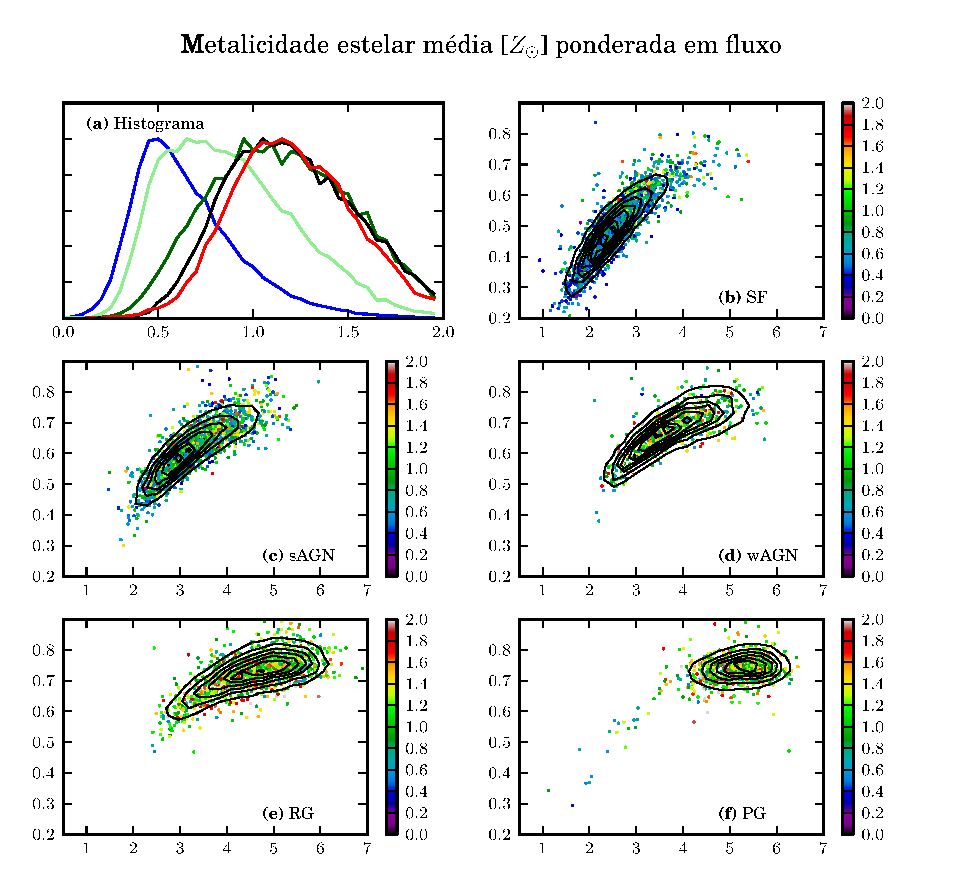
\includegraphics{figuras/uvcolor-color-am_flux-byclass.eps}
	\caption[Metalicidade estelar média ponderada em fluxo no diagrama cor--cor.]
	{O mesmo que a Figura \ref{fig:ATFluxColor}, para a metalicidade estelar média
	das galáxias, ponderada pelo fluxo.}
	\label{fig:AMFluxColor}
\end{figure}

\begin{figure}
	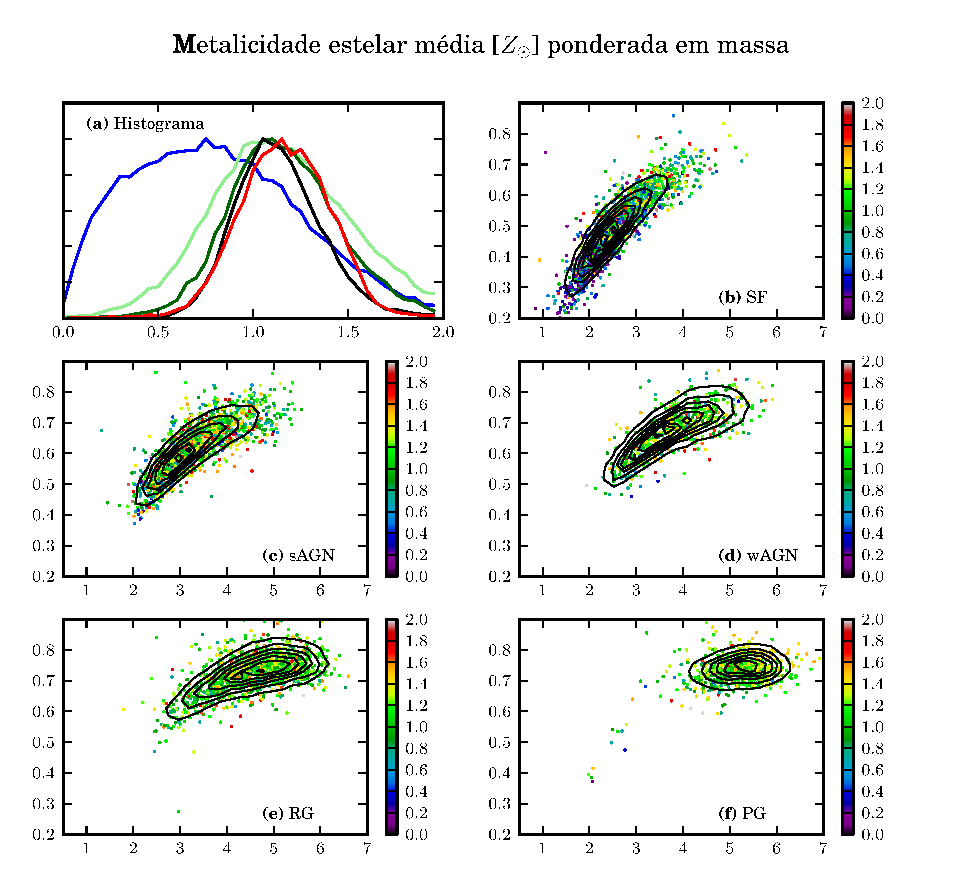
\includegraphics{figuras/uvcolor-color-am_mass-byclass.eps}
	\caption[Metalicidade estelar média ponderada em massa no diagrama cor--cor.]
	{O mesmo que a Figura \ref{fig:ATFluxColor}, para a metalicidade estelar média
	das galáxias, ponderada pela massa.}
	\label{fig:AMMassColor}
\end{figure}

A metalicidade estelar, ponderada em fluxo, das PG, RG e wAGN é em média
superior à metalicidade solar e são virtualmente indistinguíveis, conforme os
painéis (d), (e) e (f) da Figura \ref{fig:AMFluxColor}. As SF e sAGN,
respectivamente nos painéis (b) e (c) da mesma figura, por outro lado têm
metalicidades sub-solares. No diagrama cor--cor, as galáxias azuis têm em geral
metalicidade estelar mais baixa, embora não haja uma sequência tão clara quanto
para a idade estelar. A Figura \ref{fig:AMMassColor} mostra a mesma relação para
a metalicidade estelar ponderada em massa, porém neste caso as sAGN têm
metalicidade mais próxima das wAGN.

\begin{figure}
	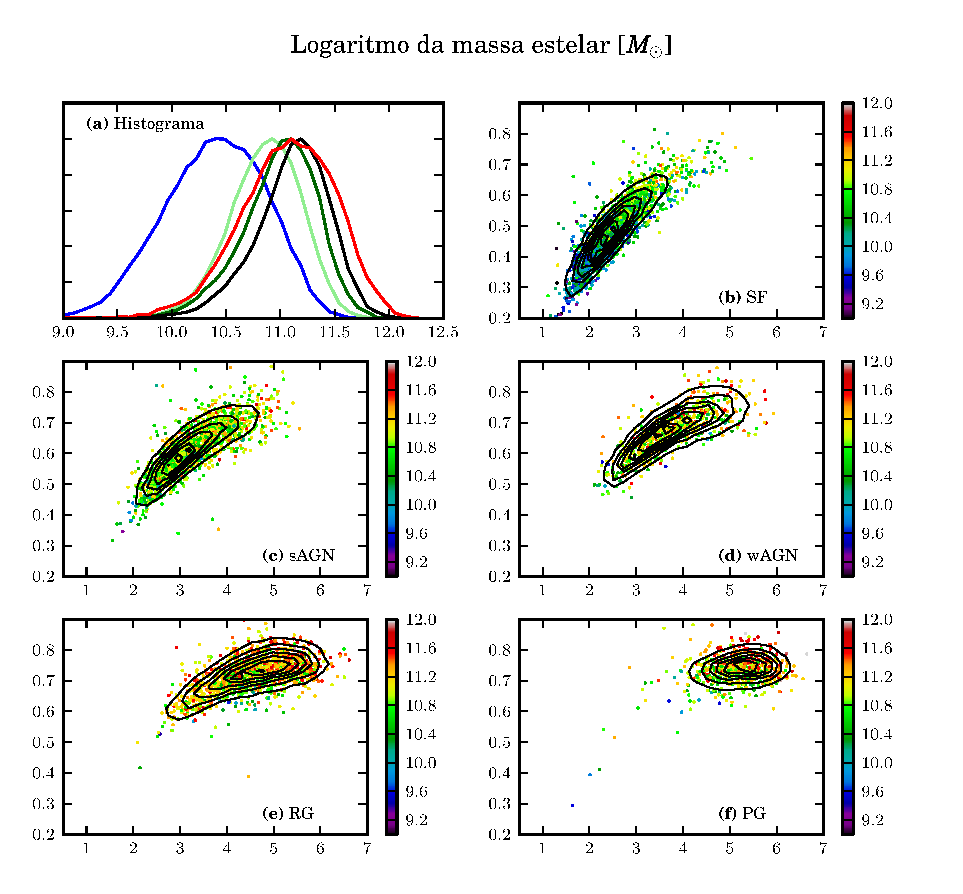
\includegraphics{figuras/uvcolor-color-mcor_gal-byclass.eps}
	\caption[Massa estelar das galáxias no diagrama cor--cor.]
	{O mesmo que a Figura \ref{fig:ATFluxColor}, para o logaritmo da massa estelar
	das galáxias em massas solares.}
	\label{fig:MCorGalColor}
\end{figure}

A massa estelar das SF é consideravelmente menor do que as outras classes
(Figura \ref{fig:MCorGalColor}). Estas têm praticamente a mesma distribuição de
massa estelar, com as sAGN ligeiramente menos massivas em média. Como visto, as
SF são em geral mais azuis, a distribuição de massa estelar no diagrama cor--cor
mostra uma certa tendência para massas menores no extremo azul.

\begin{figure}
	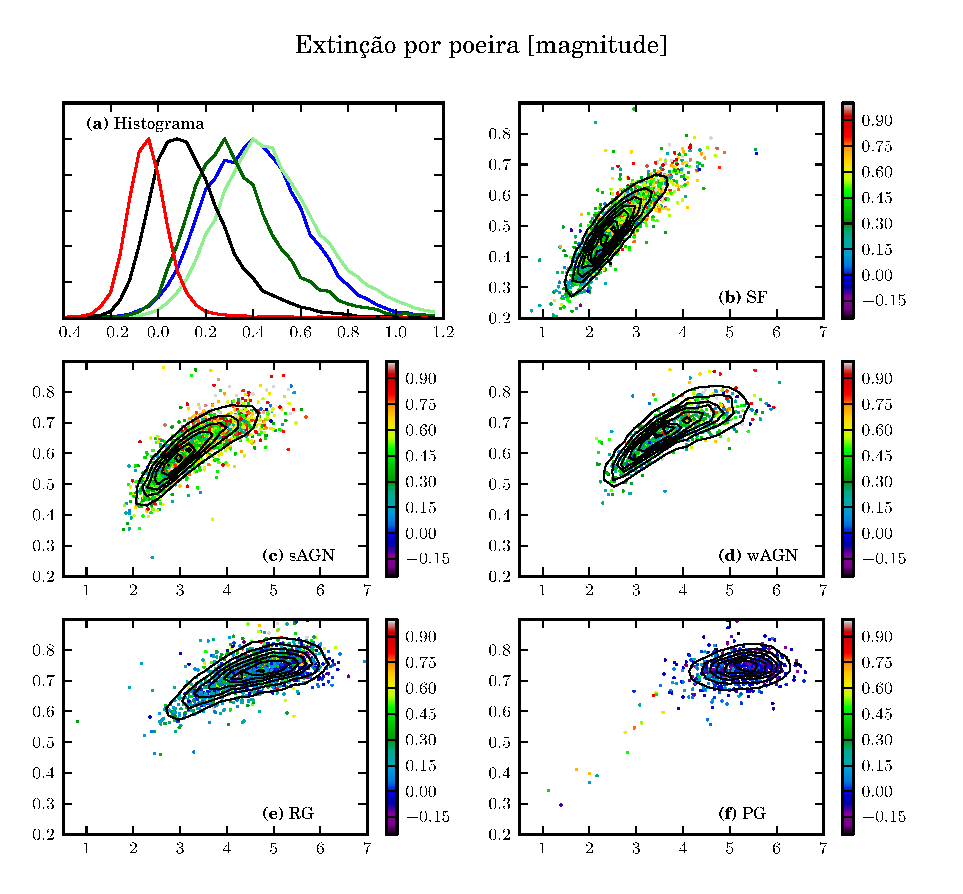
\includegraphics{figuras/uvcolor-color-AV-byclass.eps}
	\caption[Atenuação por poeira no diagrama cor--cor.]
	{O mesmo que a Figura \ref{fig:ATFluxColor}, para a atenuação por
	poeira na banda $V$ das galáxias.}
	\label{fig:AVColor}
\end{figure}

A atenuação por poeira na banda $V$ no diagrama cor--cor pode ser vista para
cada classe de galáxias na Figura \ref{fig:AVColor}. A atenuação também forma
uma sequência: PG, RG, wAGN e sAGN, em ordem crescente de atenuação, com as SF
tendo atenuação similar às sAGN. A cor também está correlacionada com a
atenuação, com galáxias azuis tendo atenuação maior do que as vermelhas. Uma
coisa que chama a atenção é o fato de haver galáxias com atenuação negativa.
Isto pode indicar que a galáxia tem populações mais vermelhas do que as
existentes na base de SSP. Como o espectro da galáxia é mais vermelho do que
todos os espectros da base, o excesso de vermelho acaba sendo compensado através
de um ``azulamento'' do espectro, que é equivalente a um avermelhamento $A_V$
negativo. Também, galáxias com $A_V$ próximo a zero e com um espectro muito
ruidoso podem ter um ajuste melhor desta forma. Este resultado só ocorre porque
$A_V$ é um parâmetro livre na síntese do \starlight.

Em geral pode-se notar que a cor UV das galáxias está relacionada de alguma
forma com as suas propriedades físicas. Para algumas propriedades, como a idade
estelar média, esta relação é bastante pronunciada. Os novos dados
observacionais, isto é, a magnitude NUV das galáxias, estão de acordo com o que
seria esperado com base numa classificação feita por linhas de emissão, e também
com a síntese feita pelo \starlight, ambos provenientes dos espectros óticos do
\SDSS. A concordância destas informações vindas de comprimentos de onda
diferentes (e {\em surveys} diferentes) fortalece a validade tanto do esquema de
classificação quanto da síntese.


% End of this chapter
